
                \begin{figure}
                    \centering
                    \begin{tikzpicture}
                        \pgfplotsset{%
                            width=1\textwidth,
                            height=0.4\textheight
                        }
                        \begin{axis}[
                            xlabel={Start temperature},
                            ylabel={Average dynamic energy (watt)},
                            ymin=0,ymax=100,
                        ]
                        
                            \addplot [mark=none, densely dashed, red]  coordinates {
                            (35, 18.18590732616388)(40, 18.369287564448882)
                            };
                            \addlegendentry{workstation - IntelPowerGadget}
                            
                            \addplot [mark=none, densely dashed, blue]  coordinates {
                            (40, 17.935803438153563)(45, 18.02230916993157)(50, 18.50229206962415)
                            };
                            \addlegendentry{workstation - HardwareMonitor}
                            
                            \addplot [mark=none, densely dashed, cyan]  coordinates {
                            (40, 13.599398769726394)(45, 14.835423341550499)(50, 15.810792920870043)(55, 13.290324089319611)
                            };
                            \addlegendentry{workstation - Clamp (win)}
                            
                        \end{axis}
                    \end{tikzpicture} 
                \caption{A graph illustrating the energy consumption of Cores for test case Nbody with regards to the temperature of the DUT, experiment \#2, (without outliers)} \label{fig:Nbody_Cores_temperature_exp2}
                \end{figure}
                